%%%%%%%%%%%%%%%%%%%%%%%%%%%%%%%%%%%%%%%%%
% Wenneker Article
% LaTeX Template
% Version 2.0 (28/2/17)
%
% This template was downloaded from:
% http://www.LaTeXTemplates.com
%
% Authors:
% Vel (vel@LaTeXTemplates.com)
% Frits Wenneker
%
% License:
% CC BY-NC-SA 3.0 (http://creativecommons.org/licenses/by-nc-sa/3.0/)
%
%%%%%%%%%%%%%%%%%%%%%%%%%%%%%%%%%%%%%%%%%

%----------------------------------------------------------------------------------------
%	PACKAGES AND OTHER DOCUMENT CONFIGURATIONS
%----------------------------------------------------------------------------------------

\documentclass[10pt, a4paper]{ctexart} % 10pt font size (11 and 12 also possible), A4 paper (letterpaper for US letter) and two column layout (remove for one column)

%%%%%%%%%%%%%%%%%%%%%%%%%%%%%%%%%%%%%%%%%
% Wenneker Article
% Structure Specification File
% Version 1.0 (28/2/17)
%
% This file originates from:
% http://www.LaTeXTemplates.com
%
% Authors:
% Frits Wenneker
% Vel (vel@LaTeXTemplates.com)
%
% License:
% CC BY-NC-SA 3.0 (http://creativecommons.org/licenses/by-nc-sa/3.0/)
%
%%%%%%%%%%%%%%%%%%%%%%%%%%%%%%%%%%%%%%%%%

%----------------------------------------------------------------------------------------
%	PACKAGES AND OTHER DOCUMENT CONFIGURATIONS
%----------------------------------------------------------------------------------------

\usepackage[english]{babel} % English language hyphenation

\usepackage{CJK}

\usepackage{microtype} % Better typography

\usepackage{amsmath,amsfonts,amsthm} % Math packages for equations

\usepackage[svgnames]{xcolor} % Enabling colors by their 'svgnames'

\usepackage[hang, small, labelfont=bf, up, textfont=it]{caption} % Custom captions under/above tables and figures

\usepackage{booktabs} % Horizontal rules in tables

\usepackage{lastpage} % Used to determine the number of pages in the document (for "Page X of Total")

\usepackage{graphicx} % Required for adding images

\usepackage{enumitem} % Required for customising lists
\usepackage{enumerate} %Required 
\setlist{noitemsep} % Remove spacing between bullet/numbered list elements

%\usepackage{sectsty} % Enables custom section titles
%\allsectionsfont{\usefont{OT1}{phv}{m}{n}} % Change the font of all section commands (Helvetica)

%----------------------------------------------------------------------------------------
%	MARGINS AND SPACING
%----------------------------------------------------------------------------------------

\usepackage{geometry} % Required for adjusting page dimensions

\geometry{
	top=1cm, % Top margin
	bottom=1.5cm, % Bottom margin
	left=2cm, % Left margin
	right=2cm, % Right margin
	includehead, % Include space for a header
	includefoot, % Include space for a footer
	%showframe, % Uncomment to show how the type block is set on the page
}

\setlength{\columnsep}{7mm} % Column separation width

%----------------------------------------------------------------------------------------
%	FONTS
%----------------------------------------------------------------------------------------

\usepackage[T1]{fontenc} % Output font encoding for international characters
\usepackage[utf8]{inputenc} % Required for inputting international characters

\usepackage{XCharter} % Use the XCharter font

%----------------------------------------------------------------------------------------
%	HEADERS AND FOOTERS
%----------------------------------------------------------------------------------------

\usepackage{fancyhdr} % Needed to define custom headers/footers
\pagestyle{fancy} % Enables the custom headers/footers

\renewcommand{\headrulewidth}{0.0pt} % No header rule
\renewcommand{\footrulewidth}{0.4pt} % Thin footer rule

\renewcommand{\sectionmark}[1]{\markboth{#1}{}} % Removes the section number from the header when \leftmark is used

%\nouppercase\leftmark % Add this to one of the lines below if you want a section title in the header/footer

% Headers
\lhead{Session \textbf{1} } % Left header
\chead{\textit{\thetitle}} % Center header - currently printing the article title
\rhead{} % Right header

% Footers
\lfoot{ME阅读材料系列} % Left footer
\cfoot{中山大学岭南学院MBA课程} % Center footer
\rfoot{\footnotesize Page \thepage\ of \pageref{LastPage}} % Right footer, "Page 1 of 2"

\fancypagestyle{firstpage}{ % Page style for the first page with the title
	\fancyhf{}
	\renewcommand{\footrulewidth}{0pt} % Suppress footer rule
}

%----------------------------------------------------------------------------------------
%	TITLE SECTION
%----------------------------------------------------------------------------------------

\newcommand{\authorstyle}[1]{{\large\usefont{OT1}{phv}{b}{n}\color{DarkRed}#1}} % Authors style (Helvetica)

\newcommand{\institution}[1]{{\footnotesize\usefont{OT1}{phv}{m}{sl}\color{Black}#1}} % Institutions style (Helvetica)

\usepackage{titling} % Allows custom title configuration

\newcommand{\HorRule}{\color{DarkGoldenrod}\rule{\linewidth}{1pt}} % Defines the gold horizontal rule around the title

\pretitle{
	\vspace{-30pt} % Move the entire title section up
	\HorRule\vspace{10pt} % Horizontal rule before the title
	\fontsize{32}{36}\usefont{OT1}{phv}{b}{n}\selectfont % Helvetica
	\color{DarkRed} % Text colour for the title and author(s)
}

\posttitle{\par\vskip 15pt} % Whitespace under the title

\preauthor{} % Anything that will appear before \author is printed

\postauthor{ % Anything that will appear after \author is printed
	\vspace{10pt} % Space before the rule
	\par\HorRule % Horizontal rule after the title
	\vspace{20pt} % Space after the title section
}

%----------------------------------------------------------------------------------------
%	ABSTRACT
%----------------------------------------------------------------------------------------

\usepackage{lettrine} % Package to accentuate the first letter of the text (lettrine)
\usepackage{fix-cm}	% Fixes the height of the lettrine

\newcommand{\initial}[1]{ % Defines the command and style for the lettrine
	\lettrine[lines=3,findent=4pt,nindent=0pt]{% Lettrine takes up 3 lines, the text to the right of it is indented 4pt and further indenting of lines 2+ is stopped
		\color{DarkGoldenrod}% Lettrine colour
		{#1}% The letter
	}{}%
}

\usepackage{xstring} % Required for string manipulation

\newcommand{\lettrineabstract}[1]{
	\StrLeft{#1}{1}[\firstletter] % Capture the first letter of the abstract for the lettrine
	\initial{\firstletter}\textbf{\StrGobbleLeft{#1}{1}} % Print the abstract with the first letter as a lettrine and the rest in bold
}

%----------------------------------------------------------------------------------------
%	SECTION
%----------------------------------------------------------------------------------------
\CTEXsetup[format={\raggedright \bfseries \LARGE \color{red}}]{section} % Specifies the document structure and loads requires packages

%----------------------------------------------------------------------------------------
%	ARTICLE INFORMATION
%----------------------------------------------------------------------------------------

\title{老头子做事总不会错} % The article title

\author{
	\authorstyle{鲁晓东\textsuperscript{1,2}} % Authors
	\newline\newline % Space before institutions
	\textsuperscript{1}\institution{中山大学岭南学院经济学系}\\ % Institution 1
	%\textsuperscript{2}\institution{University of Texas at Austin, Texas, United States of America}\\ % Institution 2
	%\textsuperscript{3}\institution{\texttt{LaTeXTemplates.com}} % Institution 3
}

% Example of a one line author/institution relationship
%\author{\newauthor{John Marston} \newinstitution{Universidad Nacional Autónoma de México, Mexico City, Mexico}}

\date{\today} % Add a date here if you would like one to appear underneath the title block, use \today for the current date, leave empty for no date
%------------加水印-------------------------------------------
\usepackage{draftwatermark}         % 所有页加水印
%\usepackage[firstpage]{draftwatermark} % 只有第一页加水印
%\SetWatermarkText{Xiaodong Lu}           % 设置水印内容
\SetWatermarkText{
\includegraphics{fig//lingnan.png}}         % 设置水印logo
\SetWatermarkLightness{0.9}             % 设置水印透明度 0-1
\SetWatermarkScale{0.5}                   % 设置水印大小 0-1    
%--------------------------------------------------------------

%----------------------------------------------------------------------------------------

\begin{document}

\maketitle % Print the title

\thispagestyle{firstpage} % Apply the page style for the first page (no headers and footers)

%----------------------------------------------------------------------------------------
%	ABSTRACT
%----------------------------------------------------------------------------------------

	
	\lettrineabstract{现在我要告诉你一个故事。那是我小时候听来的。从那时起,我每次一想到它,就似乎觉得它更可爱。故事也跟许多人一样,年纪越大,就越显得可爱,就像你们的ME老师一样,这真是有趣极了!这个故事的名字叫《老头子做事总不会错》,是丹麦作家安徒生的童话代表作之一,讲述了主人公农民通过交换虽然在利益上面吃亏,但是依然乐观开朗的故事。这个故事发表于1861年在哥本哈根出版的《新的童话和故事集》第二卷第一部。}
	




%----------------------------------------------------------------------------------------
%	ARTICLE CONTENTS
%----------------------------------------------------------------------------------------



\section*{}

\begin{figure}[t]	\centering
	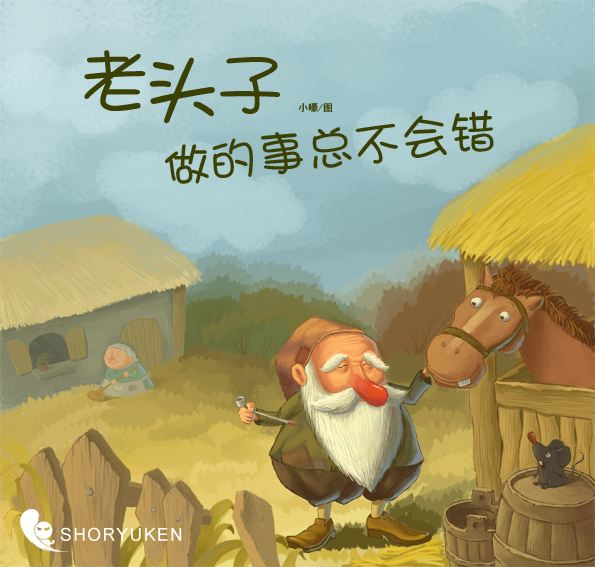
\includegraphics[scale=0.6]{fig//oldman.jpg} % Figure image
	\caption{《老头子做的事总不会错》绘本插图} % Figure caption
	\label{oldman} % Label for referencing with \ref{bear}
\end{figure}

我想你一定到乡下去过吧?你一定看到过一个老农舍。屋顶是草扎的,上面零乱地长了许多青苔和小植物。屋脊上有一个颧鸟窠,因为我们没有颧鸟是不成的。墙儿都有些倾斜, 窗子也都很低,而且只有一扇窗子是可以开的。面包炉从墙上凸出来,像一个胖胖的小肚皮。有一株接骨木树斜斜地靠着围篱。这儿有一株结结疤疤的柳树,树下有一个小水池,池里有一只母鸡和一群小鸭。是的,还有一只看家犬。它对什么来客都要叫几声。


乡下就只有这么一个农舍。这里面住着一对年老的夫妇——一个庄稼人和他的妻子。不管他们的财产少得多么可怜,他们总觉得放弃件把东西没有什么关系。比如他们的一匹马就可以放弃。它依靠路旁沟里的一些青草活着。老农人到城里去骑着它,他的邻居借它去用,偶尔帮忙这对老夫妇做点活,作为报酬。不过他们觉得最好还是把这匹马卖掉,或者用它交换些对他们更有用的东西。但是应该换些什么东西呢?


“老头子,你知道得最清楚呀,”老太婆说。“今天镇上是集日,你骑着它到城里去,把这匹马卖点钱出来,或者交换一点什么好东西:你做的事总不会错的。快到集上去吧。”

于是她替他裹好围巾,因为她做这件事比他能干;她把它打成一个双蝴蝶结,看起来非常漂亮。然后她用她的手掌心把他的帽子擦了几下。同时在他温暖的嘴上接了一个吻。这样,他就骑着这匹马儿走了。他要拿它去卖,或者把它换一件什么东西。是的,老头儿知道他应该怎样来办事情的。

太阳照得像火一样,天上见不到一块乌云。路上布满了灰尘,因为有许多去赶集的人不是赶着车,便是骑着马,或者步行。太阳是火热的,路上没有一块地方可以找到荫处。

这时有一个人拖着步子,赶着一只母牛走来,这只母牛很漂亮,不比任何母牛差。

“它一定能产出最好的奶!”农人想。“把马儿换一头牛吧——这一定很合算。”

“喂,你牵着一头牛!”他说。“我们可不可以在一起聊几句?听我讲吧——我想一匹马比一头牛的价值大,不过这点我倒不在乎。一头牛对于我更有用。你愿意跟我交换吗?”

“我当然愿意的!”牵着牛的人说。于是他们就交换了。

这桩生意就做成了。农人很可以回家去的,因为他所要做的事情已经做了。不过他既然计划去赶集,所以他就决定去赶集,就是去看一下也好。因此他就牵着他的牛去了。

他很快地向前走,牛也很快地向前走。不一会儿他们赶上了一个赶羊的人。这是一只很漂亮的羊,非常健壮,毛也好。

“我倒很想有这匹牲口,”农人心里想。“它可以在我们的沟旁边找到许多草吃。冬天它可以跟我们一起待在屋子里。有一头羊可能比有一头牛更实际些吧。“我们交换好吗?”

赶羊人当然是很愿意的,所以这笔生意马上就成交了。于是农人就牵着他的一头羊在大路上继续往前走。

他在路上一个横栅栏旁边看到另一个人;这人臂下夹着一只大鹅。

“你夹着一个多么重的家伙!”农人说,“它的毛长得多,而且它又很肥!如果把它系上一根线,放在我们的小池子里,那倒是蛮好的呢。我的老女人可以收集些菜头果皮给它吃。她说过不知多少次:‘我真希望有一只鹅!’现在她可以有一只了。——它应该属于她才是。你愿不愿交换?我把我的羊换你的鹅,而且我还要感谢你。”

对方一点也不表示反对。所以他们就交换了;这个农人得到了一只鹅。

这时他已经走进了城。公路上的人越来越多,人和牲口挤作一团。他们在路上走,紧贴着沟沿走,一直走到栅栏那儿收税人的马铃薯田里去了。这人有一只母鸡,她被系在田里,为的是怕人多把她吓慌了,弄得她跑掉。这是一只短尾巴的鸡,她不停地眨着一只眼睛,看起来倒是蛮漂亮的。“咕!咕!”这鸡说。她说这话的时候,究竟心中在想什么东西,我不能告诉你。不过,这个种田人一看见,心中就想:“这是我一生所看到的最好的鸡!咳,她甚至比我们牧师的那只抱鸡母还要好。我的天,我倒很想有这只鸡哩!一只鸡总会找到一些麦粒,自己养活自己的。我想拿这只鹅来换这只鸡,一定不会吃亏。”

“我们交换好吗?”他说。

“交换!”对方说,“唔,那也不坏!”

这样,他们就交换了。栅栏旁的那个收税人得到了鹅;这个庄稼人带走了鸡。

他在到集上去的路上已经做了不少的生意了。天气很热,他也感到累,他想吃点东西,喝一杯烧酒。他现在来到了一个酒店门口,他正想要走进去,但店里一个伙计走出来了;他们恰恰在门口碰头。这伙计背着一满袋子的东西。

“你袋子里装的是什么东西?”农人问。

“烂苹果,”伙计说。“一满袋子喂猪的烂苹果。”

“这堆东西可不少!我倒希望我的老婆能见见这个世面呢。去年我们炭棚子旁的那棵老苹果树只结了一个苹果。我们把它保藏起来;它待在碗柜一直待到裂开为止。‘那总算是一笔财产呀。’我的老婆说。现在她可以看到一大堆财产了!是的,我希望她能看看。”

“你打算出什么价钱呢?”伙计问。

“价钱吗?我想拿我的鸡来交换。”

所以他就拿出那只鸡来,换得了一袋子烂苹果,他走进酒店,一直到酒吧间里来。他把这袋子苹果放在炉子旁边靠着,一点也没有想到炉子里正烧得有火。房间里有许多客人——贩马的,贩牲口的,还有两个英国人:他们非常有钱,他们的腰包都是鼓得满满的。他们还打起赌来呢。关于这事的下文,你且听吧。

咝——咝——咝!咝——咝——咝!炉子旁边发出的是什么声音呢?这是苹果开始在烤烂的声音。

“那是什么呢?”

唔,他们不久就知道了。他怎样把一匹马换得了一头牛,以及随后一连串的交换,一直到换得烂苹果为止的这整个故事,都由他亲自讲出来了。

“乖乖!你回到家里去时,保管你的老婆会结结实实地打你一顿!”那两个英国人说。

“她一定会跟你吵一阵。”

“我将会得到一个吻,而不是一顿痛打,”农人说。“我的女人将会说:老头子做的事儿总是对的。”

“我们打一个赌好吗?”他们说。“我们可以用满桶的金币来打赌——100镑对112镑!”

“一斗金币就够了,”农人回答说。“我只能拿出一斗苹果来打赌,但是我可以把我自己和我的老女人加进去——我想这加起来可以抵得上总数吧。”

“好极了!好极了!”他们说。于是赌注就这么确定了。

店老板的车子开出来了。那两个英国人坐上去,农人也上去,烂苹果也坐上去了。不一会儿他们来到了农人的屋子面前。

“晚安,老太太。”

“晚安,老头子。”

“我已经把东西换来了!”

“是的,你自己做的事你自己知道。”老太婆说。

于是她拥抱着他,把那袋东西和客人们都忘记掉了。

“我把那匹马换了一头母牛。”他说。

“感谢老天爷,我们有牛奶吃了。”老太婆说。“现在我们桌上可以有奶做的食物、黄油和干奶酪了!这真是一桩最好的交易!”

“是的,不过我把那头牛换了一只羊。”

“啊,那更好!”老太婆说。“你真想得周到:我们给羊吃的草有的是。现在我们可以有羊奶、羊奶酪、羊毛袜子了!是的,还可以有羊毛睡衣!一头母牛可产生不了这么多的东西!

她的毛只会白白地落掉。你真是一个想得非常周到的丈夫!”

“不过我把羊又换了一只鹅!”

“亲爱的老头子,那么我们今年的马丁节的时候可以真正有鹅肉吃了。你老是想种种办法来使我快乐。这真是一个美丽的想法!我们可以把这鹅系住,在马丁节以前它就可以长肥了。”

“不过我把这只鹅换了一只鸡。”丈夫说。

“一只鸡?这桩交易做得好!”太太说。“鸡会生蛋,蛋可以孵小鸡,那么我们将要有一大群小鸡,将可以养一大院子的鸡了!啊,这正是我所希望的一件事情。”

“是的,不过我已经把那只鸡换了一袋子烂苹果。”

“现在我非得给你一个吻不可,”老太婆说。“谢谢你,我的好丈夫!现在我要告诉你一件事情。你知道,今天你离开以后,我就想今晚要做一点好东西给你吃。我想最好是鸡蛋饼加点香菜。我有鸡蛋,不过我没有香菜。所以我到学校老师那儿去——我知道他们种的有香菜。不过老师的太太,那个宝贝婆娘,是一个吝啬的女人。我请求她借给我一点。

‘借?’她对我说:‘我们的菜园里什么也不长,连一个烂苹果都不结。我甚至连一个苹果都没法借给你呢。’不过现在我可以借给她10个,甚至一整袋子烂苹果呢。老头子,这真叫人好笑!”

她说完这话后就在他的嘴上接了一个响亮的吻。

“我喜欢看这幅情景!”那两个英国人齐声说。“老是走下坡路,而却老是快乐。这件事本身就值钱。”

所以他们就付给这个种田人112镑金子,因为他没有挨打,而是得到了吻。

是的,如果一个太太相信自己丈夫是世上最聪明的人和承认他所做的事总是对的,她一定会得到好处。

请听着,这是一个故事!这是我在小时候听到的。现在你也听到它了,并且知道那个老头子做的事儿总是对的。

%---------------------------------问题
\section*{问题}
\begin{enumerate}
	\item 老头子做的“生意”都是赔钱的,是否说明他是不理性的呢?
	\item 两个英国最后损失了很多金币,他们打赌的行为是否不理性?
	\item 是否只有成功了决策才叫理性?
	\item “双十一”时候沦为“剁手党”,他们是理性的吗?
	\item 当人们说“经济学中的‘理性人假设’早被推翻了”时,人们在说什么?
\end{enumerate}

%----------------------------------------------------------------------------------------
%	BIBLIOGRAPHY
%----------------------------------------------------------------------------------------

%\printbibliography[title={Bibliography}] % Print the bibliography, section title in curly brackets

%----------------------------------------------------------------------------------------

%%%%%%%%%%%%%%%%%%%%%%%%%%%%%%%%%%%%%%%%%%%%%%%%%%%%%%%%%%%%%%%%
% 参考文献
%%%%%%%%%%%%%%%%%%%%%%%%%%%%%%%%%%%%%%%%%%%%%%%%%%%%%%%%%%%%%%%%
\small
%99为最大引用条数
\begin{thebibliography}{99}
	\setlength{\parskip}{0pt} %段落之间的竖直距离
	\bibitem{ref1} 童话世界中幸运的“老实人”——《饼干树》与《老头子做事总不会错》人物形象分析 徐宏 - 《西南农业大学学报:社会科学版》- 2012年12期
	\bibitem{ref2} 网络资料:\url{https://baijiahao.baidu.com/s?id=1578200570515459757&wfr=spider&for=pc}.
	\end {thebibliography}

\end{document}
